
\documentclass{standalone}
\usepackage{tikz}
\usetikzlibrary{arrows.meta, positioning}

\usepackage{amssymb} 
\usetikzlibrary{shapes.geometric}
\newcommand\px{0}
\begin{document}
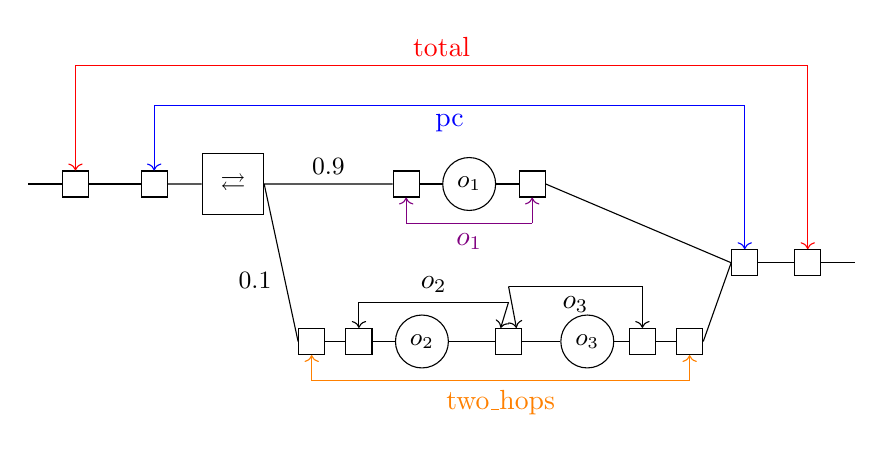
\begin{tikzpicture}[square/.style={regular polygon,regular polygon sides=4}]

    % Probability 
    \node at (\px -1, 1) [square, draw] (ss) {};
    \node at (\px, 1) [square, draw] (s) {}; 
    \node at (\px + 1, 1) [square, draw] (probab) {\small $\rightleftarrows$};
    
    \node at (\px + 3.2, 1) [square, draw] (o1s) {};
    \node at (\px + 4, 1) [circle, draw] (o3) {\small $o_1$};
    \node at (\px + 4.8, 1) [square, draw] (o1e) {};
    \node at (\px + 2, -1) [square, draw] (twos) {};
    \node at (\px + 2.6, -1) [square, draw] (o2s) {};
    \node at (\px + 3.4, -1) [circle, draw] (o4) {\small $o_2$};
    \node at (\px + 7.5, 0) [square, draw] (e) {};
    
    \node at (\px + 4.5, -1) [square, draw] (b) {};

    \node at (\px +5.5, -1) [circle, draw] (o5) {\small $o_3$};
     \node at (\px + 6.2, -1) [square, draw] (o3e) {};   
 \node at (\px + 6.8, -1) [square, draw] (twoe) {};   
    \node at (\px + 8.3, 0) [square, draw] (syse) {}; 
    
    \draw (\px - 1.6, 1) -- (ss.west);
    \draw (ss.east) -- (s.west);
    \draw (s.east) -- (probab.west);
    \draw (probab.east) -- (o1s.west) node[midway, above] {\small 0.9};
    \draw (probab.east) -- (twos.west) node[midway, below left] {\small 0.1};
    \draw (o1s.east) -- (o3.west);
    \draw (o3.east) -- (o1e.west);
    \draw (twos.east) -- (o2s.west);
    \draw (o2s.east) -- (o4.west);
    \draw (o1e.east) -- (e.west);
    \draw (o4.east) -- (b.west);
    \draw (b.east) -- (o5.west);
    \draw (o5.east) -- (o3e.west);
    \draw (o3e.east) -- (twoe.west);
    \draw (twoe.east) -- (e.west);
    \draw (e.east) -- (syse.west);
    \draw (syse.east) -- (\px + 8.9, 0);

    \draw[->, red] (\px -1, 2.5) -- (ss.north);
    \draw[red] (\px -1, 2.5) -- (\px + 8.3, 2.5) node [midway, above] {total};
    \draw[->, red] (\px + 8.3, 2.5) -- (syse.north);
    
    \draw[blue, ->] (\px, 2) -- (s.north);
    \draw[blue] (\px, 2) -- (\px + 7.5, 2) node [midway, below] {pc};
    \draw[blue, ->] (\px + 7.5, 2) -- (e.north);

    \draw[->, violet] (\px + 3.2, 0.5) -- (o1s.south);
    \draw[violet] (\px + 3.2, 0.5) -- (\px + 4.8, 0.5) node[midway, below] {$o_1$};
    \draw[->, violet] (\px + 4.8, 0.5) -- (o1e.south);

    \draw[->, orange] (\px + 2, -1.5) -- (twos.south);
    \draw[orange] (\px + 2, -1.5) -- (\px + 6.8, -1.5) node[midway, below] {two\_hops};
    \draw[->, orange] (\px + 6.8, -1.5) -- (twoe.south);

    \draw[->] (\px + 2.6, -0.5) -- (o2s.north);
    \draw (\px +2.6, -0.5) -- (\px + 4.5, -0.5) node[midway, above] {$o_2$};
    \draw[->] (\px + 4.5, -0.5) -- ([xshift=-0.1cm] b.north);

    \draw[->] (\px +4.5, -0.3) -- ([xshift=0.1cm] b.north);
    \draw (\px + 4.5, -0.3) -- (\px + 6.2, -0.3) node [midway, below] {$o_3$};
    \draw[->] (\px + 6.2, -0.3) -- (o3e.north);

\end{tikzpicture}
\end{document}
